%% ----------------------------------------------------------------------------
% CVG SA/MA thesis template
%
% Created 03/08/2024 by Tobias Fischer
%% ----------------------------------------------------------------------------
\newpage
\chapter{Experiments}

% ------- Instructions for writing the experiments section:
% Describe the evaluation you did in a way, such that an independent researcher can repeat it. Cover the following questions:
% \begin{itemize}
 % \item \textit{What is the experimental setup and methodology?} Describe the setting of the experiments and give all the parameters you have used in detail. Give a detailed account of how the experiment was conducted.
 % \item \textit{What are your results?} In this section, a \emph{clear description} of the results is given. If you produced lots of data, include only representative data here and put all results into the appendix. 
% \end{itemize}


\section{Experimental Setup}

\subsection{Datasets}

\paragraph{Hi4D.}
We evaluate on Hi4D, an indoor multi-camera dataset with two interacting people performing complex motions. Hi4D provides multi-view videos as well as ground truth meshes and poses, which enables quantitative evaluation of novel view synthesis, pose estimation, and mesh reconstruction. We follow the evaluation protocol of MultiPly \cite{multiply} for fair comparison and use the following scenes from Hi4D: \textit{pair15-fight15-view4}, \textit{pair16-jump16-view4}, \textit{pair17-dance17-view28} and \textit{pair19-piggyback19-view4}. Since our estimated cameras and SMPL-X parameters can live in a different world coordinate frame than the ground truth, we apply a camera-based world alignment using the provided camera parameters and use the same alignment consistently across all tasks, including pose and reconstruction metrics.


\paragraph{MMM.}
We also evaluate on MMM \cite{multiply} to cover scenes with more than two people and dynamic camera motion. MMM contains scenes with three to four interacting people captured with a single moving handheld camera and provides ground truth meshes and camera poses, but does not provide the full set of annotations required by all evaluation tasks. Therefore, for MMM we primarily report mesh reconstruction metrics. We follow the evaluation protocol of MultiPly and use the following scenes from MMM: \textit{dance}, \textit{lift} and \textit{walkdance}. 

\subsection{Evaluation Metrics}

\paragraph{Novel view synthesis.}
We evaluate rendering quality using PSNR and SSIM (higher is better) and LPIPS (lower is better) \cite{lpips}. PSNR measures the pixel-wise fidelity of the reconstructed image by computing the logarithmic ratio between the maximum pixel value and the mean squared error, and is reported in decibels. SSIM measures perceived structural similarity by comparing local luminance, contrast, and structure between images. LPIPS is a learned perceptual metric that compares deep features extracted by a pretrained network and correlates better with human judgement than purely pixel-based metrics.

For each Hi4D scene, we treat one camera as the source view and evaluate novel view synthesis on the remaining seven cameras. For each target camera and frame, we compute the metrics between the rendered image and the corresponding ground truth image, using the human foreground mask to restrict evaluation to pixels belonging to the people. Following MultiPly \cite{multiply}, we downscale images by a factor of two for evaluation. We then aggregate the results by averaging over all evaluation frames and all target cameras to obtain a single score per scene. Finally, we report dataset-level results by averaging these per-scene scores.

\paragraph{Pose estimation.}
We assess pose quality using MPJPE (mm) and mean vertex error (MVE, mm), as well as interaction-focused metrics: contact distance (CD, mm) \cite{yin2023hi4d} and percentage of correct depth relations (PCDR) \cite{bev} with a threshold of $0.15$m. Hi4D provides ground truth SMPL parameters, and MultiPly reports pose metrics in the SMPL space. Therefore, for fair comparison, we convert our predicted SMPL-X parameters to SMPL parameters using the official SMPL-X model transfer procedure \cite{smplx} and evaluate all pose metrics in the SMPL parameterization.

MPJPE measures the mean Euclidean distance between corresponding predicted and ground truth SMPL joints, averaged over all joints and people in the frame, where lower is better. MVE is defined analogously but computes the mean Euclidean distance between corresponding SMPL mesh vertices, and lower values indicate a more accurate reconstruction of the posed body surface. We report MPJPE and MVE in global coordinates and do not apply root alignment.

To capture interaction quality, we report contact distance (CD), which measures how well the predicted meshes reproduce inter-person contact. Given ground truth contact correspondences between the two SMPL meshes, we compute the average distance between corresponding contact points in the prediction, reported in millimeters, where lower is better. Finally, PCDR measures whether the predicted depth ordering between people matches the ground truth. For each frame, we transform the predicted and ground truth person translations to camera coordinates and derive each person's depth from the $z$ component. We then evaluate all person pairs and check whether their relative depth relation is predicted correctly under the threshold $\tau=0.15$m. Following the protocol in \cite{bev} used by MultiPly as well, we also group people into ordinal depth layers using a depth-gap threshold $\gamma=0.3$m, and treat pairs within the same layer as being at equal depth. PCDR is reported as the fraction of correctly predicted relations in a frame, where higher is better.


\paragraph{Mesh reconstruction.}
To evaluate geometry, we report volumetric IoU (V-IoU), Chamfer distance (C-$\ell_2$, cm), point-to-surface distance (P2S, cm), and normal consistency (NC). V-IoU measures the overlap between voxelized predicted and ground truth volumes, and higher values indicate better agreement. Chamfer distance measures the average closest-point distance between two point sets sampled from the predicted and ground truth surfaces, and lower values indicate more accurate geometry. P2S measures the average distance from points sampled on the predicted surface to the closest point on the ground truth surface, and lower values indicate better surface accuracy. Normal consistency evaluates agreement between surface orientations by comparing the dot product of predicted normals with the corresponding ground truth normals at nearest surface locations, and higher values indicate more consistent surface orientation.

For this evaluation, we extract meshes from the 3DGS representation using marching cubes. Before we compute the metrics, we align the reconstructed meshes to the ground truth meshes using rigid ICP (no scaling). We run ICP for 10 iterations with a convergence threshold of $10^{-4}$ and use 1000 surface samples to estimate the alignment.

For Chamfer distance, P2S, and normal consistency we estimate the metrics by sampling 1000 points uniformly from each mesh surface. Unfortunately, MultiPly does not report these evaluation hyperparameters, so we choose them ourselves and use the same settings across all methods for fair comparison. For volumetric IoU, we voxelize meshes using voxel size 0.02 with padding 0.05 around the joint bounds of predicted and ground truth meshes.

\paragraph{Instance segmentation.}
Segmentation quality is important to accurately separate dynamic humans from the static background. We therefore measure segmentation quality using intersection-over-union (IoU), recall, and F1 score.

\subsection{Implementation Details}
Unless stated otherwise, we optimize only the 3DGS parameters and keep SMPL-X parameters and camera parameters fixed. We initialize the canonical 3DGS using LHM and apply DiFix to obtain pseudo ground truth novel training views. Each person is represented by $N=40{,}000$ Gaussians.
We optimize the 3DGS parameters using AdamW with learning rate $10^{-5}$ and batch size $5$. We train for 15 epochs and use gsplat \cite{ye2025gsplat} for differentiable Gaussian rendering. To construct the training set, we generate 7 novel training view camera trajectories and subsample the original video frames by a factor of 5 (for example, 100 frames become 20 training timestamps).
For preprocessing, we use the original Hi4D image resolution, while for MMM we downsample images by a factor of 2. For runtime, preprocessing takes roughly 10 to 15 minutes per scene, and training takes roughly 15 minutes per scene on a single NVIDIA V100 GPU.

\section{Results}

% todo:
% 1. trying to see if i have access to faces apart from the upsampled points could make these much better
% 2. also i guess if improve pose i would think these results should improve as well
\subsection{Reconstruction Comparisons}
\begin{table}[!ht]
  \centering
  \caption{\textbf{Human mesh reconstruction results on Hi4D and MMM.} Best results per dataset and metric are in bold.}
  \label{tab:reconstruction_results}
  \small
  \setlength{\tabcolsep}{7pt}
  \begin{tabular}{ll
      S[table-format=1.3]
      S[table-format=1.2]
      S[table-format=1.2]
      S[table-format=1.3]}
    \toprule
    \textbf{Dataset} & \textbf{Method} & \multicolumn{1}{c}{\textbf{V-IoU} $\uparrow$} & \multicolumn{1}{c}{\textbf{C-$\ell_2$} $\downarrow$} & \multicolumn{1}{c}{\textbf{P2S} $\downarrow$} & \multicolumn{1}{c}{\textbf{NC} $\uparrow$} \\
    \midrule
    Hi4D & ECON & 0.787 & 3.72 & 3.59 & 0.746 \\
     & V2A & 0.783 & 3.02 & 2.46 & 0.775 \\
     & MultiPly & \textbf{0.816} & \textbf{2.53} & \textbf{2.34} & \textbf{0.789} \\
     & Ours & 0.560 & 4.63 & 2.86 & 0.733 \\
    \midrule
    MMM & ECON & 0.760 & 4.17 & 3.71 & 0.705 \\
     & V2A & 0.812 & 3.34 & 2.68 & 0.735 \\
     & MultiPly & \textbf{0.826} & \textbf{2.89} & \textbf{2.40} & \textbf{0.757} \\
     & Ours & 0.377 & 6.33 & 3.86 & 0.641 \\
    \bottomrule
  \end{tabular}
\end{table}

We compare our mesh reconstruction quality to MultiPly \cite{multiply} and additionally report ECON \cite{econ} and Vid2Avatar (V2A) \cite{guo2023vid2avatar} as reference baselines used in MultiPly. Across both Hi4D and MMM, MultiPly achieves the best scores across all reconstruction metrics, while our method trails and degrades further on MMM, which contains more people and dynamic camera motion. We attribute the gap mainly to two factors: first, errors in the fixed pose initialization can place the posed 3DGS in an incorrect configuration, which directly hurts volume and surface metrics; second, MultiPly reconstructs an implicit signed distance field that is designed for surface extraction, whereas our explicit 3DGS is optimized for rendering and mesh extraction via marching cubes on a density field is only an approximation. Overall, these results suggest that the current pipeline is not yet competitive for high-fidelity geometry, and that improving pose refinement and surface extraction is the most direct direction for future work.

% todo:
% 1. adding vit pose based alignment might be interesting - to see how much we get from this
% 2. optimising pose during training as well would be interesting to see how much we can gain here
% 3. replacing human3r with promt hmr would probably also help a bit
\subsection{Pose Estimation Comparisons}

\begin{table}[!ht]
  \centering
  \caption{\textbf{Human pose estimation results on Hi4D.} Best results are in bold.}
  \label{tab:pose_results_hi4d}
  \small
  \setlength{\tabcolsep}{6pt}
  \begin{tabular}{l
      S[table-format=2.1]
      S[table-format=3.1]
      S[table-format=3.1]
      S[table-format=1.3]}
    \toprule
    \textbf{Method} & \multicolumn{1}{c}{\textbf{MPJPE} $\downarrow$} & \multicolumn{1}{c}{\textbf{MVE} $\downarrow$} & \multicolumn{1}{c}{\textbf{CD} $\downarrow$} & \multicolumn{1}{c}{\textbf{PCDR} $\uparrow$} \\
    \midrule
    CLIFF & 85.7 & 102.1 & 351.7 & 0.606 \\
    TRACE & 95.6 & 115.7 & 249.4 & 0.603 \\
    MultiPly & \textbf{69.4} & 83.6 & 218.4 & \textbf{0.709} \\
    Ours & 93.9 & \textbf{77.7} & \textbf{195.8} & 0.647 \\
    \bottomrule
  \end{tabular}
\end{table}

We compare our pose estimation results to MultiPly \cite{multiply} and include for reference CLIFF \cite{li2022cliff} and TRACE \cite{trace} as reported by MultiPly. MultiPly initializes poses with TRACE, refines them using ViTPose \cite{vitpose}, and further optimizes poses during training via a photometric loss, while our method relies on the initial Human3R estimates \cite{chen2025human3r} without refinement. The results show a clear trade-off: MultiPly achieves the best MPJPE and PCDR, indicating more accurate joint locations and depth ordering, while our method achieves lower MVE and CD, indicating smaller vertex-space error and closer inter-person contact distances. A likely reason is that we keep pose fixed and do not apply 2D keypoint refinement or pose optimization during training, so residual global pose errors remain and affect joint-based metrics, while surface-based metrics can still benefit from the SMPL prior and the fixed interaction configuration. Overall, the pose results suggest that adding pose refinement and optimization is the most direct path to improve MPJPE and PCDR without sacrificing the strong contact behavior.

% todo:
% 1. having progressive refinemnt as well and showing we get better masks would make this section more meaningful, although the improvemnt would be probably small given how good sam3 is
\subsection{Instance Segmentation Comparisons}
\begin{table}[!ht]
  \centering
  \caption{\textbf{Human instance segmentation results on Hi4D.} Best results are in bold.}
  \label{tab:segmentation_results_hi4d}
  \small
  \setlength{\tabcolsep}{7pt}
  \begin{tabular}{l
      S[table-format=1.3]
      S[table-format=1.3]
      S[table-format=1.3]}
    \toprule
    \textbf{Method} & \multicolumn{1}{c}{\textbf{IoU} $\uparrow$} & \multicolumn{1}{c}{\textbf{Recall} $\uparrow$} & \multicolumn{1}{c}{\textbf{F1} $\uparrow$} \\
    \midrule
    MultiPly (Init.) & 0.943 & 0.975 & 0.984 \\
    MultiPly (Progressive) & 0.963 & \textbf{0.985} & \textbf{0.990} \\
    Ours & \textbf{0.974} & 0.982 & 0.987 \\
    \bottomrule
  \end{tabular}
\end{table}

We compare our mask segmentation quality to MultiPly, which reports results for both its initial masks from SAM1 \cite{sam1} and its progressively refined masks during training. In contrast, we do not refine masks during training and rely on the initial masks from SAM3 \cite{carion2025sam3segmentconcepts}. All methods achieve strong scores, with our method obtaining the best IoU, while MultiPly's progressive masking achieves slightly higher recall and F1. This suggests different error modes: SAM3 tends to produce cleaner average overlap, while progressive refinement reduces missed foreground pixels. Overall, segmentation quality is strong and is unlikely to be the main bottleneck, although small boundary errors can still affect downstream rendering and reconstruction.


% todo: i think here it would be interesting to compare to
% 1. some multi view video generatio method that would condition on camera parameters, e.g. sv4d2.0 - the only issue is that the camera is conntrolled via elevation deg
% 2. shape of motion - template free method, outputs 3dgs representation, so here the camera conditioning would be straight forward
% 3. would be probably good to include also comparison to guess the unseen which is 3dgs based
% 4. i could also include the results from LHM alone to have representation of the image to 3d methods
\subsection{Novel View Synthesis Comparisons}
\begin{figure}[!ht]
    \centering
    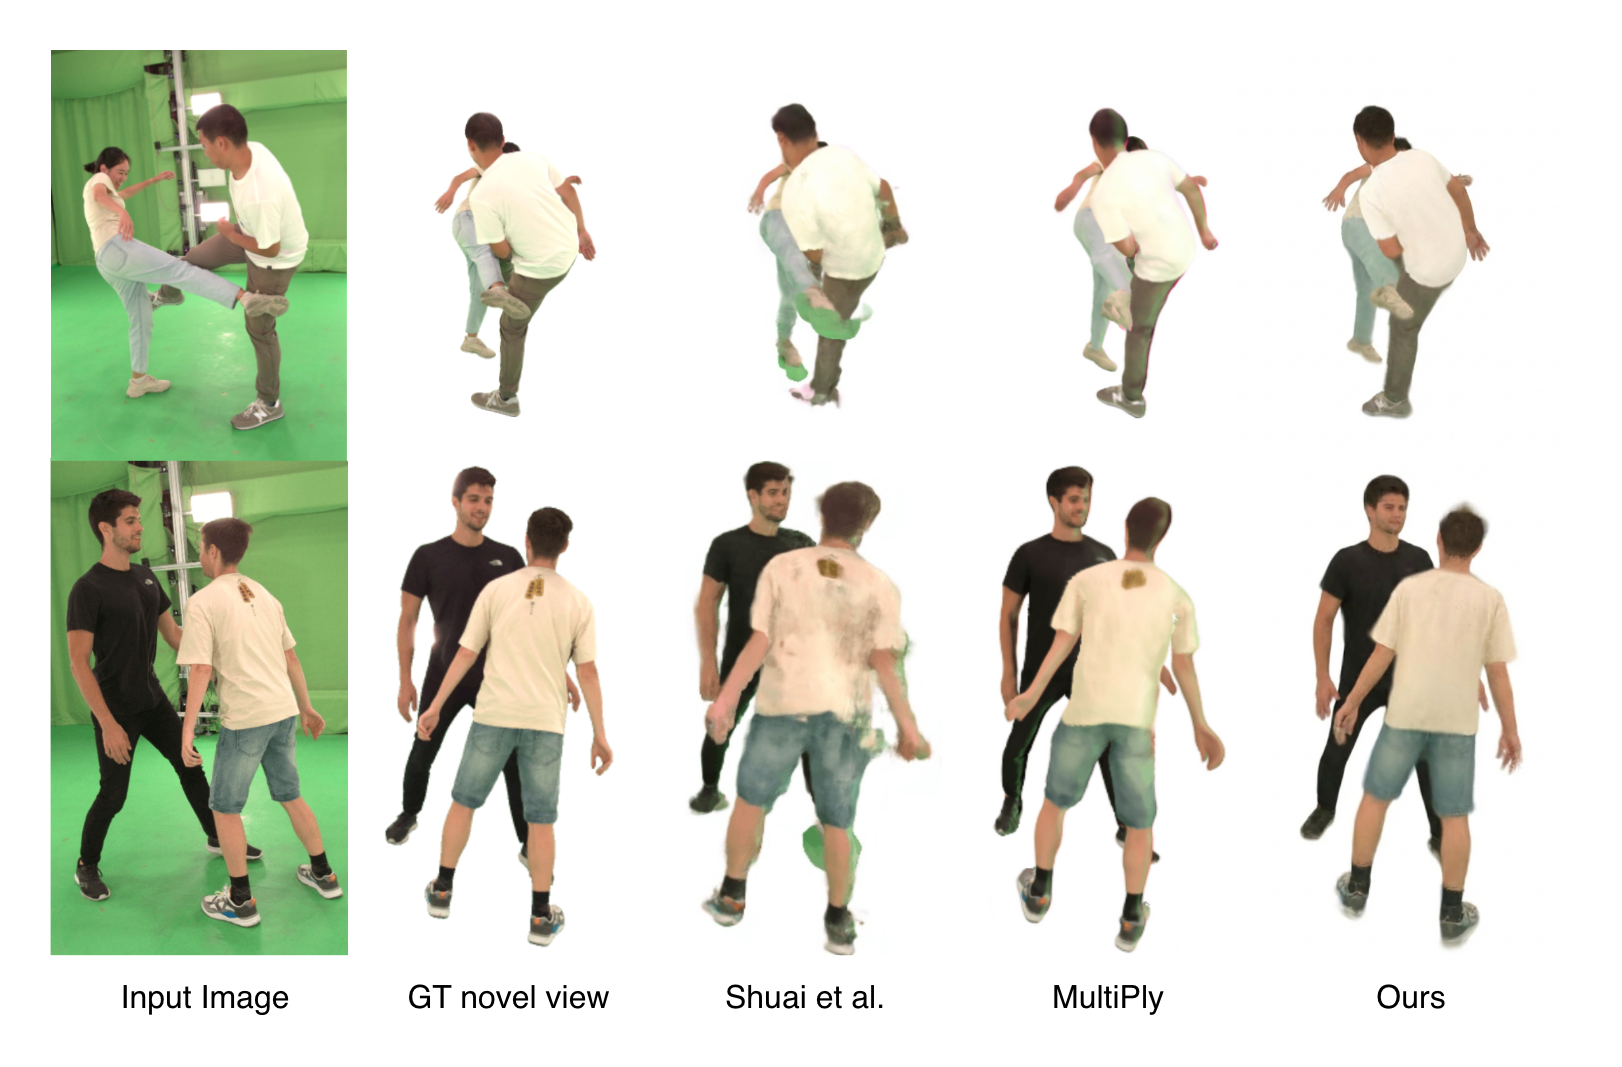
\includegraphics[width=0.8\textwidth]{figures/qual_nvs_comp.drawio.png}
    \caption{\textbf{Qualitative novel view synthesis comparison}. We show qualitative comparison to the relevant baselines on chosen scenes from Hi4D.}
    \label{fig:qual_nvs_comp}  
\end{figure}

\begin{table}[!ht]
  \centering
  \caption{\textbf{Novel view synthesis results on Hi4D.} Best results are in bold.}
  \label{tab:nvs_results_hi4d}
  \small
  \setlength{\tabcolsep}{7pt}
  \begin{tabular}{l
      S[table-format=1.3]
      S[table-format=2.1]
      S[table-format=1.4]}
    \toprule
    \textbf{Method} & \multicolumn{1}{c}{\textbf{SSIM} $\uparrow$} & \multicolumn{1}{c}{\textbf{PSNR} $\uparrow$} & \multicolumn{1}{c}{\textbf{LPIPS} $\downarrow$} \\
    \midrule
    Shuai et al. & 0.898 & 19.6 & 0.1099 \\
    MultiPly & 0.915 & \textbf{20.7} & \textbf{0.0798} \\
    Ours & \textbf{0.926} & 20.2 & 0.0872 \\
    \bottomrule
  \end{tabular}
\end{table}


In addition to MultiPly, we also compare to Shuai et al. \cite{nv_interact}, a multi-view method that was adapted by MultiPly to work in a monocular setting. Under the masked, downscaled evaluation protocol described above, our method achieves the best SSIM, while MultiPly achieves the best PSNR and LPIPS. This indicates that our renderings better preserve global structure, while MultiPly retains more pixel-level detail and perceptual fidelity. Overall, our novel view synthesis quality is competitive in terms of structural similarity, but there remains a gap in fine details compared to MultiPly.



\subsection{Ablation Studies}
An ablation study will be conducted to isolate the effect of key components, in particular (i) LHM initialization and (ii) DiFix-based view refinement. This requires rerunning per-scene optimization under matched settings and reporting results using the same evaluation protocol as in Tables~\ref{tab:nvs_results_hi4d}--\ref{tab:reconstruction_results}. The goal is to quantify which components primarily drive novel view synthesis improvements versus the remaining gap in mesh reconstruction.
